\textcolor{red}{[I think in the introduction we need to say that thermohaline mixing models have evolved over the years from dimensional analysis-based models (Kippenhahn) to 3d simulation based ``empirical" models (Traxler) to physics-based (Brown) but we don't need to explain beyond that.]}

Expressed in terms of typical stellar structure variables, the stability of the temperature gradient is given by the Schwarzschild criterion:
\begin{equation} \label{eq:Schwarzschild}
    \gradrad - \gradad < 0,
\end{equation}
\textcolor{red}{[paraphrase this sentence]} where the temperature gradient $\grad \equiv d \ln P / d \ln T$ (pressure $P$ and temperature $T$) is $\gradad$ for an adiabatic stratification and $\gradrad$ if all the flux is carried radiatively. 
The statement that the density gradient is strong enough to ensure stability by the Ledoux criterion despite the inversion of the mean molecular weight is
\begin{equation} \label{eq:Ledoux}
    \gradrad - \gradad - \frac{\phi}{\delta}\gradmu < 0.
\end{equation}
\textcolor{red}{[paraphrase this sentence]} The Ledoux criterion includes the effects of the composition gradient $\gradmu = d\ln\mu/d\ln P$ (mean molecular weight $\mu$), where $\delta = -(\partial \ln \rho / \partial \ln T)_{P,\mu}$ and $\phi = (\partial \ln \rho / \partial \ln\mu)_{P,T}$ (density $\rho$).

The stabilizing influence of the temperature gradient relative to the destabilizing influence of the $\mu$ gradient is often given in terms of the density ratio $R_0$, defined as
\begin{equation} \label{eq:R0}
    R_0 \equiv \frac{\grad - \gradad}{\frac{\phi}{\delta} \gradmu},
\end{equation}
where $R_0 < 1$ implies the $\mu$ gradient is sufficiently strong to drive convection, and $R_0 > 1$ implies the fluid is stably-stratified (i.e.~no convection) \textcolor{red}{[I'm being REAL careful not to say $R_0 > 1$ is Ledoux-stable, because of the $\grad$ in Eq.~\eqref{eq:R0} vs the $\gradrad$ in Eq.~\eqref{eq:Ledoux}]}. 
As reviewed by [cite Garaud review 2018], fluids with $R_0 > 1$ can be prone to double-diffusive instabilities whenever the thermal diffusivity $\kappa_T$ is greater than the compositional diffusivity $\kappa_\mu$. Specifically, the instability driving thermohaline mixing acts whenever
\begin{equation} \label{eq:R0_condition}
1 < R_0 < 1/\tau,
\end{equation}
[cite Stern 1960, I'm pretty sure] where
\begin{equation} \label{eq:tau}
    \tau \equiv \kappa_\mu/\kappa_T.
\end{equation}
Note that typical values of $\tau$ in stellar radiation zones are $10^{-6}$ or smaller, meaning even very slightly destabilizing $\mu$ gradients [how do I make it more obvious that this means ``big $\mu$ over small $\mu$"?] can drive thermohaline mixing, even when the temperature gradient is far from being convectively unstable.

The simplicity of criterion Eq.~\eqref{eq:R0_condition} makes the necessary conditions for thermohaline mixing in stellar interiors readily identifiable. 
Indeed, sites of thermohaline mixing and possible implications have been identified in stars across the HR diagram, from [blah] to [blah] to [blah] [I have a list... will dig it up later]. 
However, predicting the efficiency of thermohaline mixing is much more challenging. 
Due to the diffusive, small-scale nature of thermohaline mixing, a diffusive approximation is commonly taken for the turbulent mixing of chemicals and heat, so that the total mixing of chemical species, say, is given by the sum of the molecular diffusivity and some turbulent mixing coefficient \Dth (the turbulent mixing of heat is typically assumed to be negligible relative to radiative diffusion). 
This quantity can be converted to the compositional Nusselt number $\mathrm{Nu}_{\mu}$ in the fluid dynamics literature using the formula $\Dth = (\mathrm{Nu}_{\mu} - 1)\kappa_\mu$. 
We refer to any model that predicts \Dth as a function of stellar structure variables (e.g.~gradients and molecular diffusivities of chemicals and heat) as a (parameterized) mixing model or mixing prescription. 
Such mixing prescriptions, when implemented in stellar evolution models such as the MESA software instrument, can be used to predict the effects of thermohaline mixing in stars across the HR diagram.

Efforts to develop thermohaline mixing prescriptions for use in modeling stellar interiors date back to the 1970's \citep{ulrich_1972}, and have ranged in sophistication from arguments based on dimensional analysis, to more involved analytical derivations informed by hydrodynamic simulations. 
The reader is again referred to [Garaud 2018] for a comprehensive review of efforts to predict mixing efficiency -- here, we briefly summarize the most commonly used and more recently developed prescriptions.

%Of the mixing models implemented in MESA, the earliest is due to \citet{ulrich_1972} and \citet{kippenhahn_etal_1980} \textcolor{red}{[check refs]}

%The density ratio is defined \citep{ulrich_1972}
%Do this in terms of N^2
%\begin{equation}
%    R_\rho = \frac{\nabla_T - \nabla_{\rm{ad}}}{{\nabla_\mu}},
%\end{equation}
%where $\nabla_T$ is the logarithmic temperature gradient, $\nabla_{\rm{ad}}$ is its adiabatic value, and $\nabla_\mu$ is the Ledoux composition gradient term.
%Throughout this section, we report mixing efficiency assuming that thermohaline mixing can be modeled as a diffusivity with diffusion coefficient $\Dth$; this quantity can be converted to the Nusselt number $\mathrm{Nu}_{\rm{th}}$ in the fluid dynamics literature using the formula $\Dth = (\mathrm{Nu}_{\rm{th}} - 1)\kappa_\mu$, where $\kappa_\mu$ is the compositional diffusivity. 

The default \textcolor{red}{[no longer default apparently. earliest? most commonly used?]} thermohaline mixing model in the MESA software instrument \citep{mesa2} was originally derived by \citet{ulrich_1972, kippenhahn_etal_1980}.
%Thermohaline mixing is treated as a diffusion process, with a diffusion coefficient
Using arguments based on dimensional grounds and assumptions about the shape and motion of fluid ``blobs", they predicted a mixing efficiency of the form
\begin{equation} \label{eq:Dth-kipp}
    \Dth = C_t \kappa_T R_0^{-1},
\end{equation}
\citep[see Eq.~(5) of][]{charbonnel_thermohaline_2007}
where $C_t$ is a free parameter, with plausible values ranging from $C_t = 658$ \citep{ulrich_1972} to $C_t = 12$ \citep{kippenhahn_etal_1980}. 
\citet{charbonnel_thermohaline_2007} used a value of $C_t = 1000$ in stellar evolution models and found chemical mixing trends that were broadly \textcolor{red}{[With some exceptions I think? Double check]} consistent with observational data from \citet{Gratton2000}.

Equation \eqref{eq:Dth-kipp} is implemented in MESA as
\begin{equation} \label{eq:Dth-kipp-MESA}
    \Dth = \alpha_{\rm{th}} \frac{3 K}{2\rho C_P}R_0^{-1}
\end{equation}
\citep[see Eq.~(14) of][]{mesa2}. 
Here, $\alpha_{\rm{th}}$ is a dimensionless efficiency parameter, $K$ is the radiative conductivity, $\rho$ is the density, and $C_P$ is the specific heat at constant pressure. 
Based on previous theoretical arguments in the literature, \citet{mesa2} suggested a plausible range of efficiency parameters as $1 \lesssim \alpha_{\rm{th}} \lesssim 667$ \textcolor{red}{[note: Cantiello and Langer claim this 667 value is equivalent to the $C_t = 1000$ value used by \citet{charbonnel_thermohaline_2007}]}, with a default value of $2$ \textcolor{red}{[Meridith rephrase the preceding sentence please]}. 

\textcolor{red}{[Adrian says please don't read past here]}

\textcolor{red}{[Need to pick either $C_t$ or $\alpha_\mathrm{th}$ and just stick with it from here on out rather than bouncing back and forth]}

\textcolor{red}{[Don't forget to note that Kippenhahn model sucks for not capturing $\Dth \to 0$ as $r \to 1$!]}

\textcolor{red}{[Consider mentioning Denissenkov 2010 model]}

While 1D stellar evolution models from \citet{charbonnel_thermohaline_2007} using $C_t = 1000$ \citep[consistent with the efficiency argued by][]{ulrich_1972} reproduced trends that are consistent with observational data from \citet{Gratton2000}, these values were orders of magnitude larger than the efficiency of thermohaline mixing put forth by, e.g., \citet{kippenhahn_etal_1980}. 
As reviewed by [cite Garaud 2018], this broad range of plausible efficiency parameters motivated the use of multidimensional simulations by multiple groups as a form of numerical experiment to more precisely estimate mixing efficiency [cite Dennisenkov; Traxler a or b I forget]. 
%\citet{traxler_etal_2011} and \citet{brown_etal_2013} performed 3D hydrodynamic simulations across a broad range of parameters and broadly found that the mixing efficiency parameter required in \citet{charbonnel_thermohaline_2007} to find agreement with observations was orders of magnitude larger than what is found in simulations, suggesting thermohaline mixing may be unable to explain observations of extra mixing.
\citet{traxler_etal_2011} and \citet{brown_etal_2013} performed 3D hydrodynamic simulations across a broad range of parameters and developed mixing prescriptions that fit their simulations. 
They found that mixing efficiency is most easily discussed in terms of $r$.
\citet{traxler_etal_2011} derived a mixing law by fitting an analytic function to their simulations.
They define the reduce density ratio, $r \equiv (R_0 - 1)/(\tau^{-1} - 1)$, where $\tau = \kappa_\mu/\kappa_T$ is the ratio of compositional to thermal diffusivity.
They find that
\begin{equation} \label{eqn:trax_model}
   \Dth = \kappa_{\mu}\sqrt{\frac{\mathrm{Pr}}{\tau}}\left(a e^{-br}[1 - r]^c\right),
\end{equation}
where $\mathrm{Pr} = \nu / \kappa_T$ with $\nu$ the viscosity, and they find $a = 101 \pm 1$, $b = 3.6 \pm 0.3$, and $c = 1.1 \pm 0.1$.



\citet{brown_etal_2013} note that the model in Eqn.~\ref{eqn:trax_model} performs well at high $R_\rho$, but underestimates mixing at low $R_\rho$, particularly in the stellar regime of low Pr and $\tau$.
They develop a semi-analytical model for thermohaline mixing,
\begin{equation}
    \Dth = \kappa_{\mu}C^2\frac{\lambda^2}{\tau l^2(\lambda + \tau l^2)},
    \label{eqn:brown_model}
\end{equation}
where $\lambda$ is the growth rate of the fastest growing linearly unstable mode, $l$ is its horizontal wavenumber, and $C \approx 7$ is a universal constant which they fit to simulation data.
Obtaining $\lambda$ and $l$ requires solving a cubic and quadratic equation (their Eqns.~19 and 20).

These new implementations are used in \citep{bauer_bildsten_2019} and other works.

(cite) paper is the paper that implements these new models in MESA and it's been there since r(put revision here)


\citet{harrington} build on the model of \citet{brown_etal_2013} by including magnetic fields and find that magnetism can increase mixing efficiency.
They utilize the same Eqn.~\ref{eqn:brown_model} but define the velocity of the instability $\hat{w}_f^2 = \lambda^2/l^2$ for clarity. 
Their Eqn.~32 provides an expression for $\hat{w}_f^2$ which depends on the magnitude of the magnitude field $B_0^2$.
This expression has two asymptotic limits, in which $\hat{w}_f^2 \propto B_0^2$ when $B_0$ is large, and which reduces exactly to the model of \citet{brown_etal_2013} when $B_0$ is small.
(this is a new model that is not yet implemented in MESA).


There has been other work regarding multi-D models of thermohaline mixing \citep{denissenkov_2010, denissenkov_merryfield_2011}, but 2D thermohaline behaves very differently from 3D thermohaline \citep{garaud_brummell_2015}, and so we do not consider that set of data in this work.

\citet{lattanzio_etal_2015} tested one or multiple of these models in a bunch of different codes on the RGB and found X.
In this paper, we will determine if observations are capable of probing the differences between these different models are not.

\begin{figure}
    \centering
    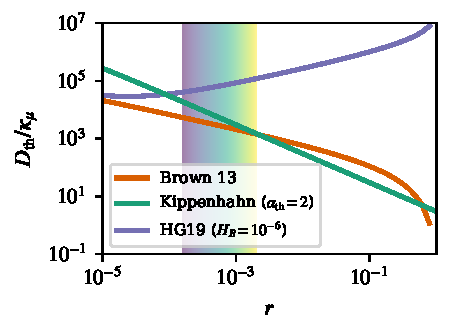
\includegraphics[width=\columnwidth]{Nu_models_comparison.pdf}
    \caption{\textcolor{red}{[Todo: Write caption.]}}
    \label{fig:parameterization_compare}
\end{figure}

\textbf{Adrian}: Start making this plot
Do you need to discuss here? or cite previous work? include plot of Nu vs R0 with the different model/theory predictions, mark simulations, like you did for bring a plot [AF: assuming I finally wrap up my in-prep paper with Pascale, we can just cite that paper and throw in those Nu vs R0 plots]
